
\documentclass[showpacs,showkeys,preprint,prd,nofootinbib,linenumbers,12pt]{revtex4-1}

\usepackage{graphicx} % This is already loaded by the atlasnote class
% Just use it to include your plots!

\usepackage{rotating}
\usepackage{amsmath}
% use less space for subfigures
\usepackage{epstopdf}
\usepackage{multirow}
\usepackage{xspace}
\usepackage{rotating}
\usepackage{longtable}
\usepackage{multirow}
\usepackage{cancel}


\usepackage[breaklinks=true]{hyperref}
\hypersetup{
  colorlinks=true,
  linkcolor=blue,
  citecolor=blue,
  urlcolor=blue
}

\makeatletter
\renewcommand*\env@matrix[1][*\c@MaxMatrixCols c]{%
  \hskip -\arraycolsep
  \let\@ifnextchar\new@ifnextchar
  \array{#1}}
\makeatother



\graphicspath{{./fig/}}
\usepackage{array,tabularx,epsfig,mathrsfs,graphicx,rotating}
\usepackage{ifthen}
\usepackage{amsfonts}

\usepackage{subfigure}

\subfigcapskip = -0.7cm

\newcommand{\beq}{\begin{equation}}
  \newcommand{\eeq}{\end{equation}}
\newcommand{\F}{\mathrm{F}}
\chardef\til=126
\newcommand{\mev}{{\,\mathrm{MeV}}}
\newcommand{\gev}{{\,\mathrm{GeV}}}
\newcommand{\tev}{{\,\mathrm{TeV}}}
\newcommand{\pythia}{{\sc Pythia8}\xspace}

\def\pt{\ensuremath{p_{\mathrm{T}}}}
\def\ptRes{\ensuremath{\pt^{\mathrm{truth}}-\pt^{\mathrm{reco}}}}
\def\etaRes{\ensuremath{\eta^{\mathrm{truth}}-\eta^{\mathrm{reco}}}}
\def\phiRes{\ensuremath{\phi^{\mathrm{truth}}-\phi^{\mathrm{reco}}}}
\def\mRes{\ensuremath{m^{\mathrm{truth}}-m^{\mathrm{reco}}}}
\def\deltaRecoTruth{\ensuremath{\Delta(\mathrm{reco},\mathrm{truth})}}

% Draft version: if given, adds draft version on front page, a
% 'DRAFT' box on top of each other page, and line numbers to easy
% commenting. Comment or remove in final version.
% \version{1.1}

% \bibliographystyle{aipnum4-1}


% Journal: adds a 
% \journal{Phys. Lett. B} 
\begin{document}

\preprint{ANL-HEP-XXXXX}

% \hfill \today

\date{May 9, 2019}
% \hfill \today

\vspace{2.5cm}

%%%%%%%%%%%%%%%%%%%%%%%%%%%%%%%%%%%%%%%%%%%%%%%%%%%%%%%%%%%%%%% 
\title{
  Replication of detector simulations using supervised machine learning 
}
%%%%%%%%%%%%%%%%%%%%%%%%%%%%%%%%%%%%%%%%%%%%%%%%%%%%%%%%%%%%%%% 


\author{D. Benjamin, S. Chekanov, W. Hopkins, Y. Li, J. R. Love,}
\affiliation{
  HEP Division, Argonne National Laboratory,
  9700 S.~Cass Avenue, Argonne, IL 60439, USA 
}% 



\begin{abstract}

\end{abstract}


\maketitle

\section{Action items for editors}
\begin{itemize}
\item What $R$-parameter are we using? $R=0.4$ or $R=0.5$? (Sergei)
\item Sergei and Walter need to check they are doing the same matching of truth and reco jets (what is the $\Delta R$?). (Sergei/Walter)
\item Need to align parameters of unbinned and binned NNs. (Sergei/Walter)
  \begin{itemize}
  \item Why are we using different activation functions (ReLU vs sigmoid) in the hidden layers?
  \item Why do we have different dimensions for the output 100 vs 200?
  \item For the unbinned preprocessing, are we removing resolution outliers?
  \end{itemize}
\item Fix missing references (Doug).
  \begin{itemize}
  \item ReLU reference?
  \item Madgraph reference (can take this from stop0L paper)?
  \end{itemize}
\item Write something about the hyperparameters (Ying).
  \begin{itemize}
  \item Maybe rerun the hyperparameter scan again?
  \end{itemize}
\item Normalize binned NN $\eta$ comparison histograms to really see shape differences. 
\item Write conclusion (Jeremy)
  \begin{itemize}
  \item Focus on truth smearing replacement and how this is automated.
  \end{itemize}
\item Should we add CPU performance comparison?
  \begin{itemize}
  \item TruthSmearingFunctions for 1M jets vs our method?
  \end{itemize}
\item Should we do a MET and mt comparison?
  \begin{itemize}
  \item This really only makes sense within ATLAS.
  \end{itemize}
\end{itemize}

%%%%%%%%%%%%%%%%%%%%%%%%%%% 
\section{Introduction}
%%%%%%%%%%%%%%%%%%%%%%%%%%% 

A cornerstone of particle collision experiments is Monte Carlo (MC) simulations of physics processes followed  by simulations of detector responses. With increased complexity of such experiments, such as those at the Large Hadron Collider (LHC), the detector simulations become increasing complex and time consuming.  For example, the time required to simulate Geant4 hits [] and to reconstruct from such hits physics objects (electrons, muons, taus, jets) requires a factor 100-1000  more CPU time than the creation of typical Monte Carlo events that represent physics processes according to theoretical models (``truth level'' MC event generation).  A possible method to speed up simulations of detector responses is to apply neural networks (NN) trained using the actual Geant4-based simulations, and use such supervised NN for transforming truth-level MC objects (jets and other identified particles) to objects modified by detectors (``detector-level'').  

A typical simulation of detector response stochastically modifies positions and energies of particles and jets created by MC generators at the ``truth-level''. Another important component of such simulations is to introduce additional particles due to misconstructing energy deposits in active detector volumes  (examples include misreconstructed electrons or photons which are, in fact, hadronic jets, etc.). The latter effects  represent a significant complication for the so-called ``fast'' or ''parameterized'' detector simulations, such as Delphes \cite{deFavereau:2013fsa}.
Nevertheless, fast simulations is proven to be a vital tools for physics performance studies.

One advantage of fast simulations based on machine learning is that the neural networks can automatically learn the features introduced by detailed full simulations, therefore, handcrafting smearing parameters represent resolutions and inefficiencies, as it was done in Delphes and other fast simulations, is not required. A neural network trained using realistic detector simulation should memorize the transformation from the truth-level to the detector level without interference from analyzers. Another advantage is that the NN approach can introduce a complex interdependence of variables which is currently difficult to implements in parameterized fast simulations. Finally, we expect that NN approach will be faster than the current fast simulations (this will be described later).

As a first step towards fast detector simulations using machine learning techniques, it is instructive to investigate how a transformation from the ``truth-level'' MC to ``detector-level'' objects can be performed, leaving aside the question of introducing objects that are created by misreconstructions.

\section{Traditional parameterized fast simulations}

In abstract terms, a typical variable $f_i$ that characterizes a particle/jet, such as transverse momentum (\pt), pseudorapidity ($\eta$), can be viewed as a  multivariate transform $F$ of the original variable $\xi_1^T$ at truth-level:

$$
\xi_1 = F (\xi_1^T, \xi_2^T, \xi_3^T, ...\xi_N^T).
$$
Generally, such a transform  depends on several other variables $\xi_2^T$ ..  $\xi_N^T$ characterizing this (or other) objects at the truth level.   For example, the extent at which jet transverse momentum, \pt\ is modified  by a detector depends on the original truth-level transverse momentum ($\xi_1^T=p_T^T$), pseudorapidity $\eta$,  flavor of jets and other effects that can be inferred from the truth level. For example, if particular detector modules in the azimuthal angle ($\phi$) are not active, this would introduce an additional dependence of this transform on $\phi$.
% A more difficult case when other objects produced an event can influence  the transformation of $\xi_1$ from $\xi_1^T$.
Typical fast (``parameterized'') simulations ignores the full range of correlations between the variables. In most cases, the above transform is reduced to a single variable, or two (as in the case of Delphes fast simulations where energy resolution of clusters depend on the original energies of particles and their positions in $\eta$). In order to take into account correlations between  multiple parameters characterizing transformations to the detector level, the following steps have to be undertaken:

\begin{itemize}

\item
  create a grid in the hypercube with the dimension $N_b^N$, where $N_b$ is the number of histogram bins for the distributions $f_1-f_i^N$  representing ``resolution'' smearing. This can be done numerically, using frequencies, or using analytically using ``resolution functions''.

\item
  calculate ``efficiencies'' that model losses of particles/jets for each variable.

\end{itemize}

It should be pointed that the calculation speed for parameterized fast simulations of one variable that depends on $N$ other variables at the truth level depends  as $N_b^N$ since each object at the truth level should be placed inside the grid defined by $N_b$ bins. Therefore, complex parameterisations of resolutions and efficiency's for $N>2$ becomes CPU intensive. 

%%%%%%%%%%%%%%%%%%%%%%%%%%%%%%%%%%%%%%%%%%%%% 
\section{Machine learning approach for fast simulation}
%%%%%%%%%%%%%%%%%%%%%%%%%%%%%%%%%%%%%%%%%%%%% 

Unlike the traditional approach for fast simulation using parameterized density functions for resolution variables and probability values for efficiency, a neural network approach offers an opportunity to formulate this problem in terms of neural-network nodes and their connections that scale as $N_b^N \cdot N$, which can speed up the fast simulations and, at the same time, can be used for learning more complex full simulations in an automated way.

In the case of objects, such as jets, a typical truth-level input are jet transverse momentum, $\eta$, $\phi$ and jet mass $m$, while the output
is an array of output nodes that represent the binned probability density function (pdf) of the resolution for a single variable (such as jet \pt). 
The output can also include a node that specifies the efficiency, i.e. a variable that is either 0 (e.g. a jet did not pass the detector acceptance) or 1 (a jet was within the detector acceptance). Additional input variables can be jet flavor at the truth level, jet radius etc., i.e. any variable that 
can influence the output of such neural network. Figure~\ref{ann_example} shows a schematic representation of the NN architecture for modelling detector response for a single output variable. In this example, we show a single hidden layer (in principle, the NN can also be deep with several hidden layers)

\begin{figure}[h]
  \includegraphics[width=0.8\textwidth]{nn_example.png}
  \caption{A schematic representation of the NN architecture for modelling the detector response to truth-level input variables.}
  \label{ann_example}
\end{figure}


%%%%%%%%%%%%%%%%%%%%%%%%%%%%%%%%%%%%%%%%%%%%% 
\section{Monte Carlo simulated event samples}
%%%%%%%%%%%%%%%%%%%%%%%%%%%%%%%%%%%%%%%%%%%%% 

Monte Carlo events used for this analysis were generated using the Madgraph generator~\cite{madgraph}. The simulated process was $t\bar{t}+jets$, which give a high rate of jets and lepton. In addition, multijet events were added to increase the statistics at high \pt\ jets. % does multijet really add high stats?
Hadronic jets were reconstructed with the {\sc FastJet} package~\cite{fastjet} using the anti-$k_T$ algorithm \cite{Cacciari:2008gp} with a distance parameter of 0.5.  The detector simulation was performed  with the Delphes package \cite{deFavereau:2013fsa} with the ATLAS-like detector geometry. 
The event samples used in this paper, before and after the fast simulation, are  available from the HepSim database~\cite{Chekanov:2014fga}. In this paper only the transformation from truth-level jets to detector-level jets was performed, however the methodology should be object agnostic. 

The distributions of quantities used as the input for the NN, \pt, $\eta$\, $\phi$, $m$, are shown in Figure~\ref{fig:nnInputsPrescaling}.

\begin{figure}[h]
  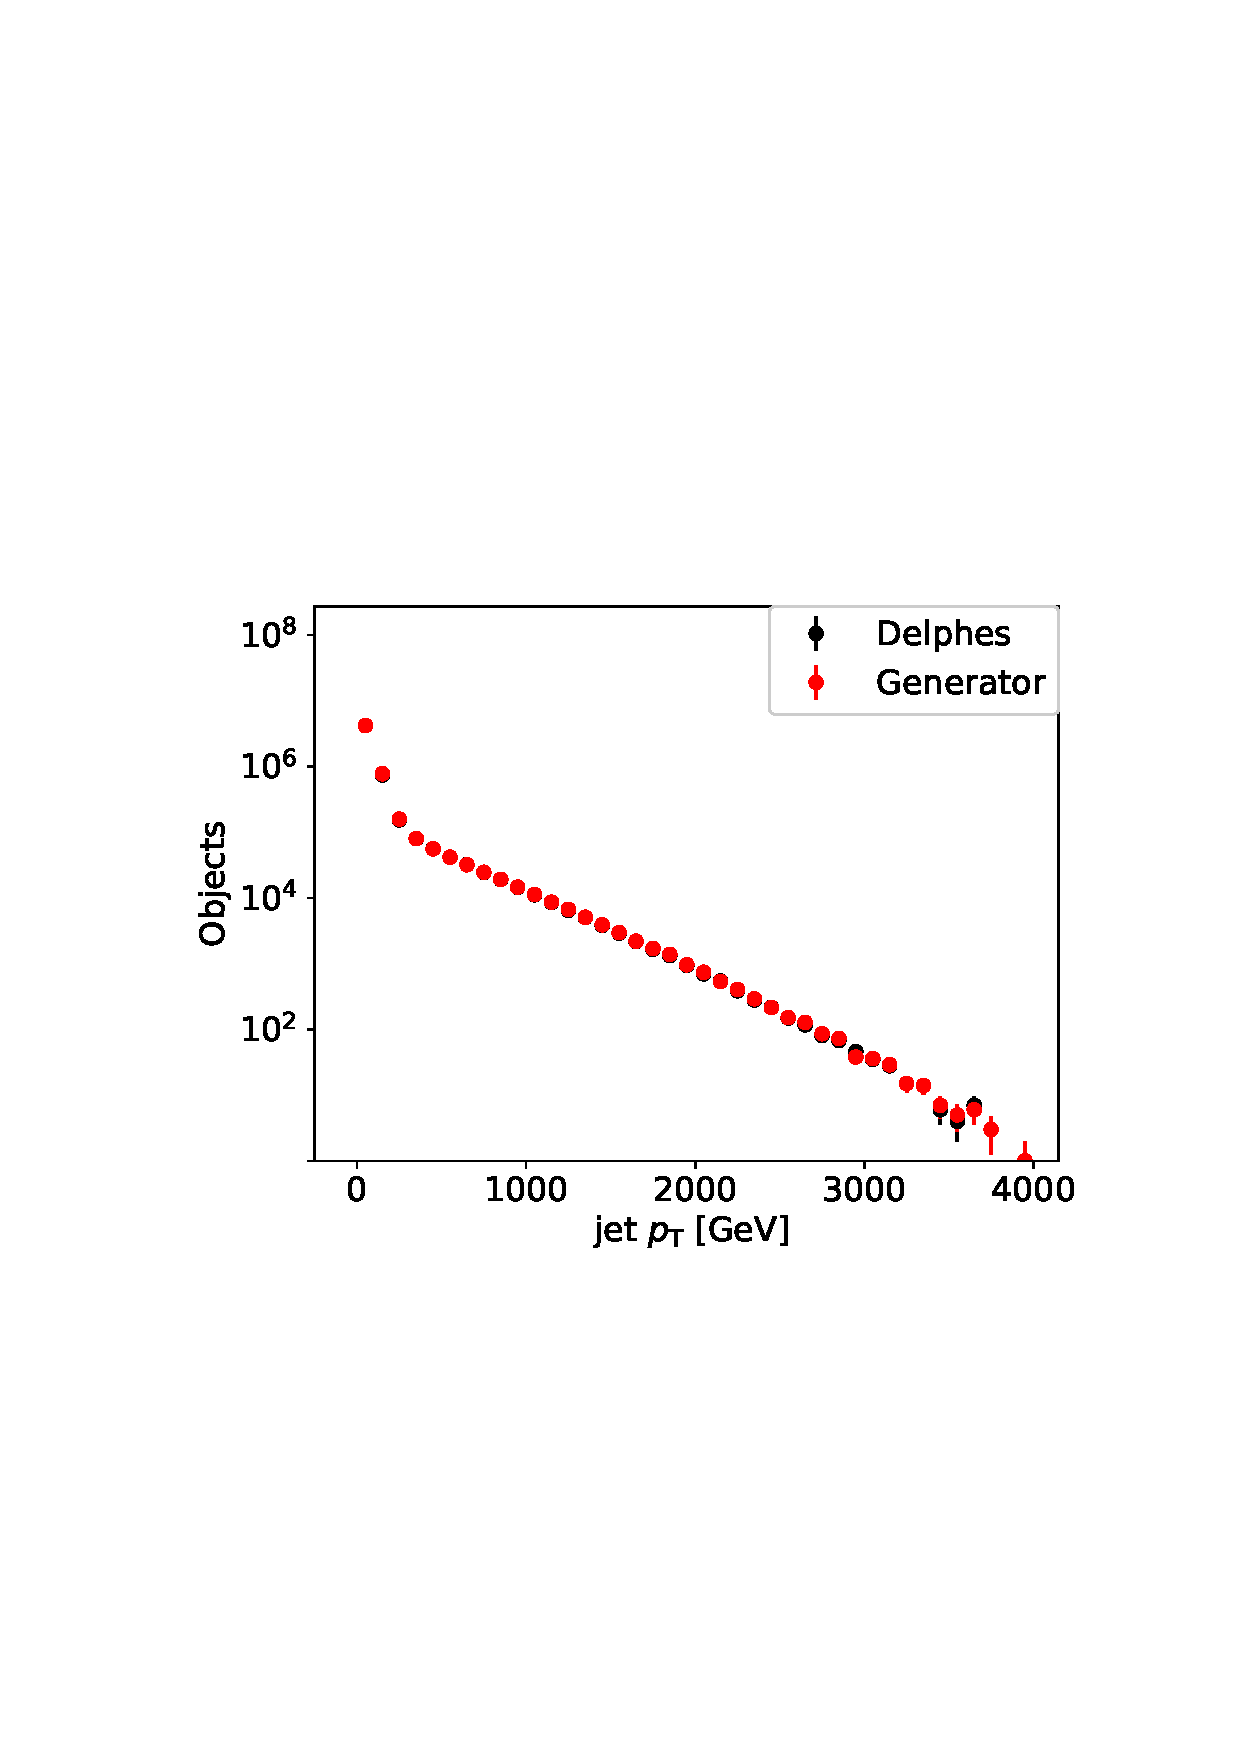
\includegraphics[width=0.48\textwidth]{jet_pT_prescaling_log.pdf}
  \includegraphics[width=0.48\textwidth]{jet_m_prescaling_log.pdf}\\
  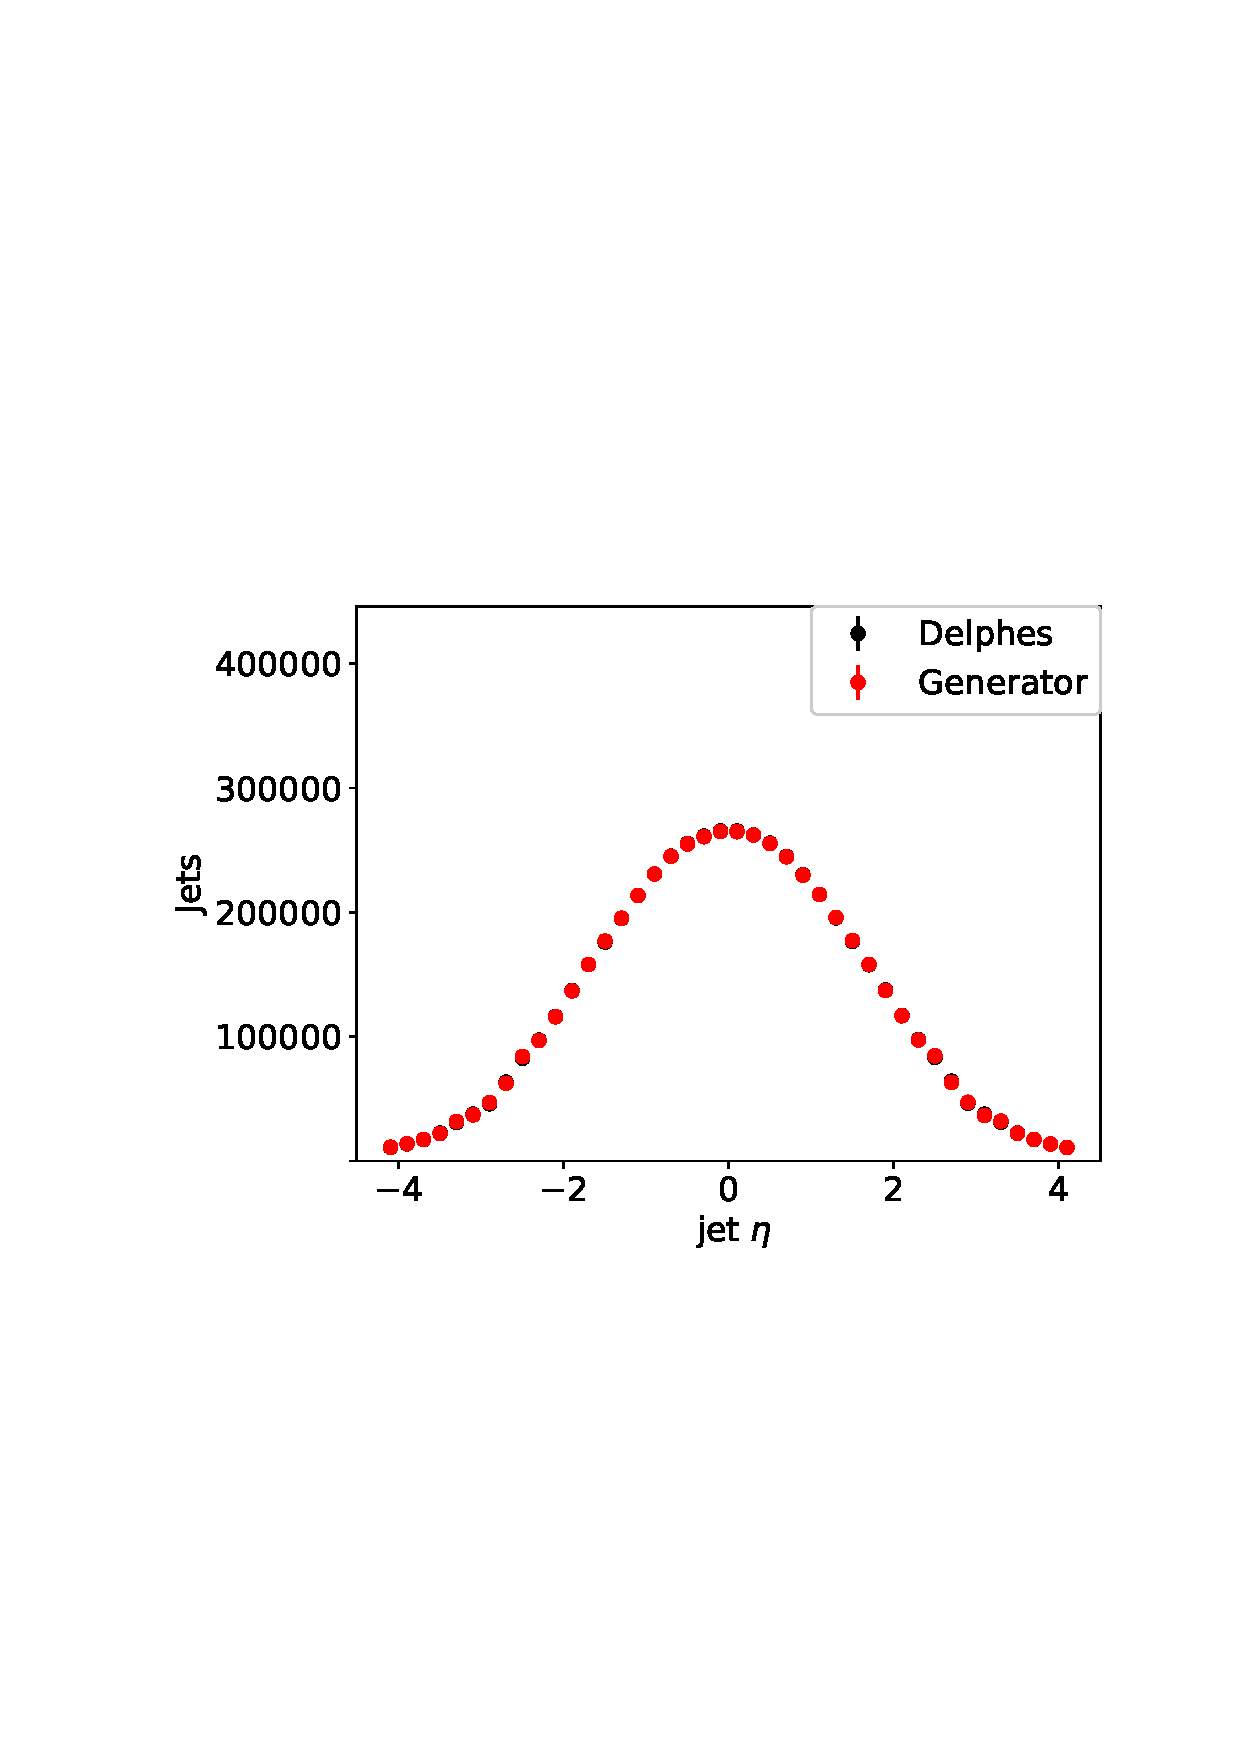
\includegraphics[width=0.48\textwidth]{jet_eta_prescaling.pdf}
  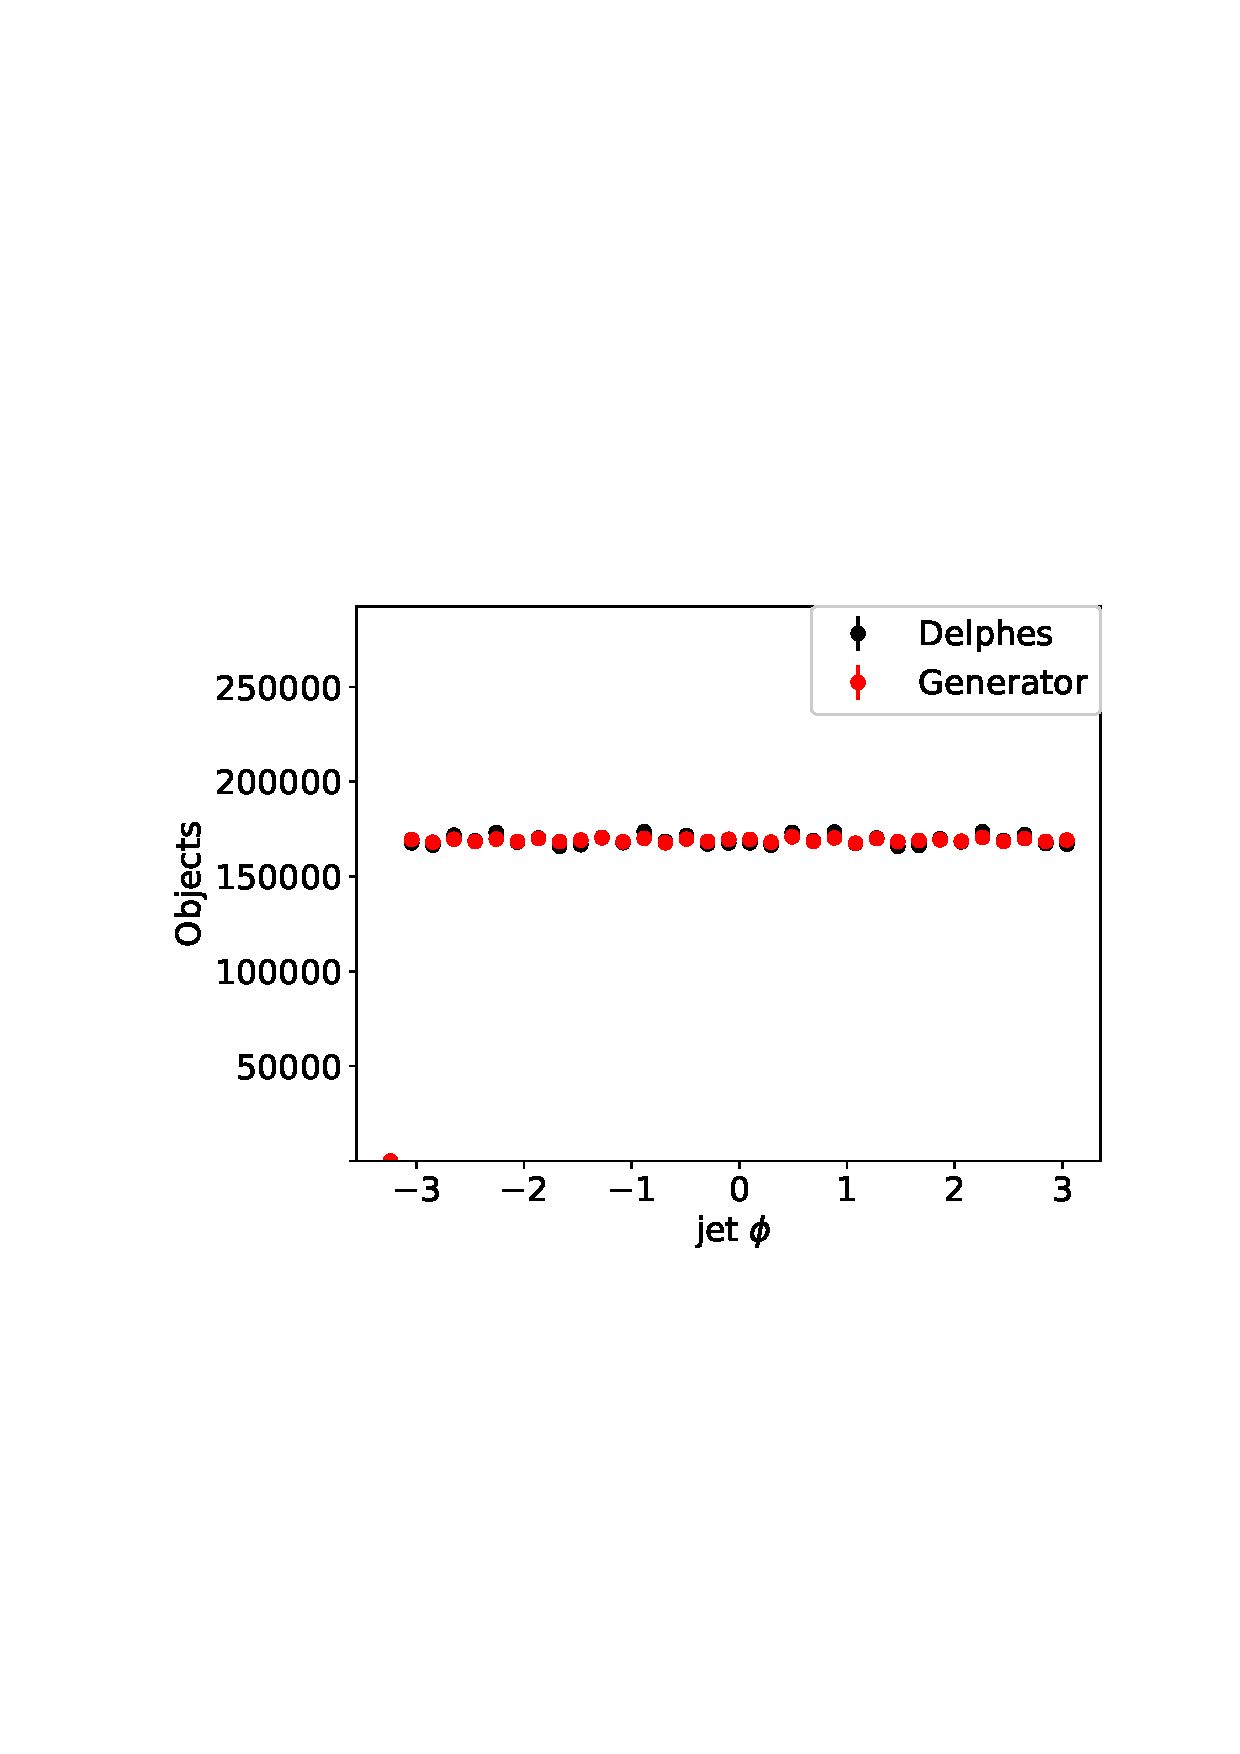
\includegraphics[width=0.48\textwidth]{jet_phi_prescaling.pdf}
  \caption{Input variable shapes for truth-level (red) and detector-level quantities (black).}
  \label{fig:nnInputsPrescaling}
\end{figure}

To facilitate gradient descent in all direction of the input variables, the input variables are all scaled to be in the range [0,1]. This avoids the \pt\ and the mass from having a disproportional affect on the training of the NNs. The output variables, consisting \ptRes, \etaRes, \phiRes, \mRes, are also scaled to have values between 0 and 1 and are shown in Figure~\ref{fig:deltaTarget}. Only object that 
are within the 1$^{\mathrm{st}}$ and 99$^{\mathrm{th}}$ percentile of each of the resolution distributions are considered in this study since objects outside this range are typically not used in physics analyses.

\begin{figure}[h]
  \includegraphics[width=0.48\textwidth]{pTRes_bounds_scaled.pdf}
  \includegraphics[width=0.48\textwidth]{mRes_bounds_scaled.pdf}\\
  \includegraphics[width=0.48\textwidth]{etaRes_bounds_scaled.pdf}
  \includegraphics[width=0.48\textwidth]{phiRes_bounds_scaled.pdf}
  \caption{Differences between truth-level and detector-level quantities after scaling so that the difference is in the range [0,1].}
  \label{fig:deltaTarget}
\end{figure}

\section{Neural network structures}

Two approaches when using the input variables are considered: one bins the input variables into 20 bins for each variable (we will called this the ``binned NN'') while the other leaves the input variables unbinned (this will be referred to as the ``unbinned NN''.
For the binned case, the network structure consists of an input layer with 4*20 nodes, one fully connected hidden layer with 100 nodes and an output layer with 201 nodes. The first 200 nodes represent the bins in jet resolution (\ptRes, \etaRes, \phiRes, \mRes), and one node is added, which either has a value of 0 and 1, represents the probability that the given input jet passes the detector acceptance and reconstruction. The binning of the output reduces a regression problem to a multi-categorization problem which simplifies and reduces the required network parameters. The NN uses sigmoid activation function for all layers. After the training, the output NN nodes contain 201 values representing the probability density distribution for the jet resolution function which can be used to generate shifts in the truth-level quantity due to the detector smearing effects.

In the case of the unbinned inputs, the outputs are binned to have 101 bins with the first bin for the first feature representing the acceptance and reconstruction inefficiency, similar to the binned NN case. {\color{red}mention what happens when there are multiple truth jets within a reco jet}. The binned output variables are shown in Figure~\ref{fig:deltaTarget}. 
As with the binned NN, an NN is trained for each feature, i.e. an NN exists for \pt, $m$, $\eta$, and $\phi$, individually, resulting in four NNs. The binned NNs consist of five layers with 100 nodes with each node having a ReLu [cite relu] activation function. The output layer has 101 nodes with a softmax activation function. The NN is trained over 20 epochs with batch size 1000. 

%%%%%%%%%%%%%%%%%%%%%%%%%%%%%%%%%%%%%%%%%%%%% 
\section{Results}
%%%%%%%%%%%%%%%%%%%%%%%%%%%%%%%%%%%%%%%%%%%%% 

The results for the binned NN training compared to the default Delphes fast simulation (used for the NN training)
are shown in Fig.~\ref{plot_ptres_eta_binned}.
To test whether the NN learned correlations between input parameters and the resolutions, the jets were divided into central ($|\eta|<2$ and forward ($|\eta|>2$ jets, then the \pt\ resolutions were compared between the two regions for both the Delphes jets as well as the NN-generated jets. These two regions in detectors typically have different jet \pt\ resolutions and thus the \pt\ resolution is correlated with the $\eta$. The trained binned NN describes the Delphes simulations well.
In particular, the dependence of jet \pt\ resolution is well modeled for different $\eta$ regions,
which is an indication that the NN learns correlations between input variables. It is also important to note that the jet efficiency included in Delphes can be reproduced by the NN with a $1\%$ accuracy.

\begin{figure}[htb]
  \includegraphics[width=0.48\textwidth]{plot_ptres_eta.pdf}
  \includegraphics[width=0.48\textwidth]{plot_ptres_all.pdf}
  \caption{Left: NN-generated jet \pt\ resolutions for central (black) and forward (red) jets for Delphes (circles) and NN-generated jets (dashed line).
  Right: The standard deviation of the \ptRes\ as a function of \pt for Delphes (black) and the NN (red).}
  \label{fig:plot_ptres_eta_binned}
\end{figure}


The learned resolution pdfs learned by the unbinned NN are compared to the Delphes resolutions in Fig.~\ref{fig:nnRes}.

\begin{figure}[htb]
  \includegraphics[width=0.48\textwidth]{jet_pTRes.pdf}
  \includegraphics[width=0.48\textwidth]{jet_mRes.pdf}\\
  \includegraphics[width=0.48\textwidth]{jet_etaRes.pdf}
  \includegraphics[width=0.48\textwidth]{jet_phiRes.pdf}
  \caption{Resolutions for the jet \pt, mass, $\eta$, $\phi$. The red dots correspond to the NN output summed over the entire test sample while the black dots correspond to resolutions from Delphes. The first bin of the \pt\ pdf is used to quantifiy the inefficiency of the reconstruction. }
  \label{fig:nnRes}
\end{figure}


The truth-level quantities are corrected using the NN generated pdfs resulting in NN generated objects. A comparison between truth-level, detector-level, and NN-generated features is shown in Fig.~\ref{fig:nnVsDelphes}. The agreement between detector-level and NN-generated features is within XX\%. As with the binned NN, figure~\ref{fig:plot_ptres_eta_unbinned} shows that the NN reproduces the difference in resolutions for central and forward jets. 

\begin{figure}[htb]
  \includegraphics[width=0.48\textwidth]{jet_pT_genVsReco_origScale_test_log.pdf}
  \includegraphics[width=0.48\textwidth]{jet_m_genVsReco_origScale_test_log.pdf}\\
  \includegraphics[width=0.48\textwidth]{jet_eta_genVsReco_origScale_test.pdf}
  \includegraphics[width=0.48\textwidth]{jet_phi_genVsReco_origScale_test.pdf}
  \caption{NN-generated jet \pt, mass, $\eta$, $\phi$ compared to truth-level and detector-level jet features. }
  \label{fig:nnVsDelphes}
\end{figure}

\begin{figure}[htb]
  \includegraphics[width=0.48\textwidth]{jet_pTResLowEta.pdf}
  \includegraphics[width=0.48\textwidth]{jet_pTResOrigScale_std.pdf}
  \caption{Left: NN-generated jet \pt\ resolutions for central (black) and forward (red) jets for Delphes (circles) and NN-generated jets (dashed line).
  Right: The standard deviation of the \ptRes\ as a function of \pt for Delphes (black) and the NN (red).}
  \label{fig:plot_ptres_eta_unbinned}
\end{figure}

\section{Hyperparameter scan}

\section{Performance consideration?}
For the binned NN, the training of one variable typically takes 30 min using 16 parallel processes.

\section{Conclusion}

\section*{Acknowledgments}
The submitted manuscript has been created by UChicago Argonne, LLC, Operator of Argonne National Laboratory (“Argonne”). Argonne, a U.S.  Department of Energy Office of Science laboratory, is operated under Contract No. DE-AC02-06CH11357. The U.S. Government retains for itself, 
and others acting on its behalf, a paid-up nonexclusive, irrevocable worldwide license in said article to reproduce, prepare derivative works, distribute copies to the public, and perform publicly and display publicly, by or on behalf of the Government.  The Department of Energy will provide public access to these results of federally sponsored research in accordance with the 
DOE Public Access Plan. \url{http://energy.gov/downloads/doe-public-access-plan}. Argonne National Laboratory’s work was funded by the U.S. Department of Energy, Office of High Energy Physics under contract DE-AC02-06CH11357. 



%%%%%%%%%%%%%%%%%%%%%% references %%%%%%%%%%%%%%%%%%%%%%%%%%%%%%
% \clearpage
\section*{References}
\bibliography{references}


\end{document}